\section{Integer Case}


In this section, we will be treating the initial value problem (i.v.p.)
\begin{equation}\label{eq:iode}
\begin{cases}
    y'= f(t,y)&\\ y(0)=y_0\quad t\in[0,T]&
\end{cases}
\end{equation}
It is important to acknowledge that these numerical procedures can only treat first order ordinary differential equations. For solving higher order ordinary differential equations, the model has to be converted to an state-space representation (system of first order differential equations. In further sections, this methodology will be explained.

\subsection{Euler's Method}\label{sec:euler}
Euler's method \cite{euler} is the most basic procedure for solving ordinary differential equations. It takes advantage of the Taylor expansion of a function $f$, given by
\begin{equation}
y(t+h)=\sum_{n=0}^{\infty}\dfrac{y^{(n)}(t)}{n!}h^n=y(t)+hy'(t)+\dfrac{h^2}{2!}y''(t)+\dfrac{h^3}{3!}y'''(t)+\dots
\end{equation}
For $h\ll1$, we have $h^n\rightarrow0$ for $n\geq2$. Therefore,
\[y(t+h)\approx y(t)+hy'(t)=y(t)+hf(t,y(t))\]
\begin{equation}\label{eq:euler}
    y_{i+1}\approx y_i+hf(t_i,y_i)
\end{equation}


With expression \eqref{eq:euler}, a discrete approximation for the initial value problem \eqref{eq:iode} can be obtained, where $h$ is known as the step size for the algorithm. Note that this method only requires the previous approximation to calculate the next one; and, in order to calculate the first one, the initial conditions are applied. Remark: the Euler's method is a first-order numerical method since it only calculates the approximation for the next iteration. In the following section, we will explain how Euler's method works.

\subsubsection{Visualization}
\noindent Taking a closer look to Euler's method, it can be observed that equation \eqref{eq:iode} is an expression for the slope of the solution at any point $(t_i,y_i)$; therefore, if we were to calculate the next point $(t_{i+1},y_{i+1})$, we set $t_{i+1}=t_i+h$ and the $y_{i+1}$ is obtained by moving along the line with slope given by equation \eqref{eq:iode} throughout a time $h$. Formally this line would be $y=mt+b$ where $m=f(t_i,y_i)$ and $b=y_i$.

Let us present what we have already mentioned graphically:
\begin{figure}[H]
    \centering
    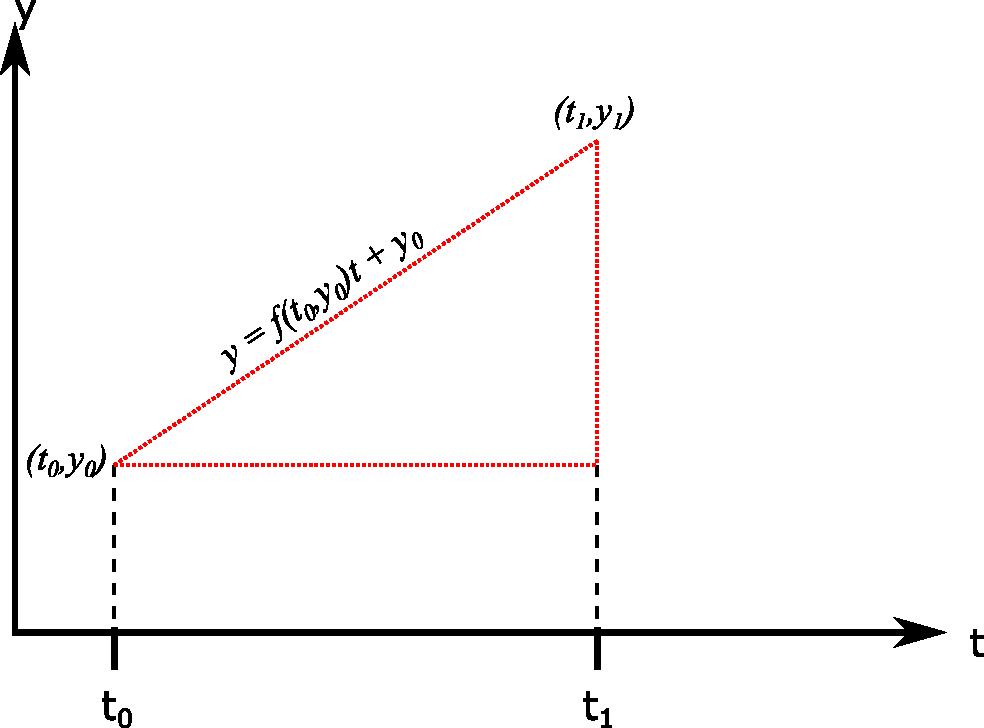
\includegraphics[scale=0.4]{files/graphicEuler.pdf}
    \caption{Visualization of Euler's method.}
    \label{fig:visualEuler}
\end{figure}

\subsubsection{Examples}
\begin{exmp} \label{ex:r_e}
Solve the following initial value problem using Euler's method \cite{exampleeuler}.
\begin{equation}
\begin{cases}
    y'+2y=2-e^{-4t}&\\ y(0)=1\quad t\in[0,2.5]&
\end{cases}
\end{equation}\label{eq:exeuler}
\end{exmp}
Throughout some calculus, the exact solution is
\begin{equation}
    y(t)=1+\dfrac{1}{2}e^{-4t}-\dfrac{1}{2}e^{-2t}
\end{equation}
For Euler's method, let us rewrite equation \eqref{eq:exeuler} as 
\begin{equation*}
    y'=2-e^{-4t}-2y
\end{equation*}
Now that we have the same form as the initial value problem \eqref{eq:iode}, let us apply Euler method with $f(t,y)=2-e^{-4t}-2y$ and $h=0.5$ for illustration purposes. In this case, we want to approximate the first five terms of the solution. Hence,
\begin{align*}
    y_0 =& y(0) = 1\\
    y_1 =& y_0+hf(t_0,y_0)= 1 + (0.5)\left[2-e^{-4\cdot0}-2(1)\right]=0.5\\
    y_2 =& y_1+hf(t_1,y_1) = 0.5 + (0.5)\left[2-e^{-4\cdot0.5}-2(0.5)\right]=0.9323\\
    &\qquad\qquad\qquad\qquad\qquad\qquad\vdots
\end{align*}
Following this procedure, one can obtain the results shown in table \ref{tab:euler}; this table shows the real value as well.

\begin{table}[H]
\centering
\begin{tabular}{cccc}
\hline
\textbf{i} & \textbf{t} & \textbf{Euler} & \textbf{Real} \\ \hline
0          & 0          & 1.0000         & 1.000         \\
1          & 0.5        & 0.5000         & 0.8837        \\
2          & 1          & 0.9323         & 0.9414        \\
3          & 1.5        & 0.9908         & 0.9763        \\
4          & 2          & 0.9987         & 0.9910        \\
5          & 2.5        & 0.9998         & 0.9966        \\ \hline
\end{tabular}
\caption{Comparison between the approximation and the real values.}
\label{tab:euler}
\end{table}
Notice that the approximation slightly differs from the real value, due to the large step size selected, though the general behavior of the solution is achieved; it is important to mention that the stationary state is successfully approximated since the differential equation describes an stable system.

In order to obtain better results, the step size can be reduced, leading to the following results, shown in figure (\ref{fig:taut}).

\begin{figure}[H]
    \centering
    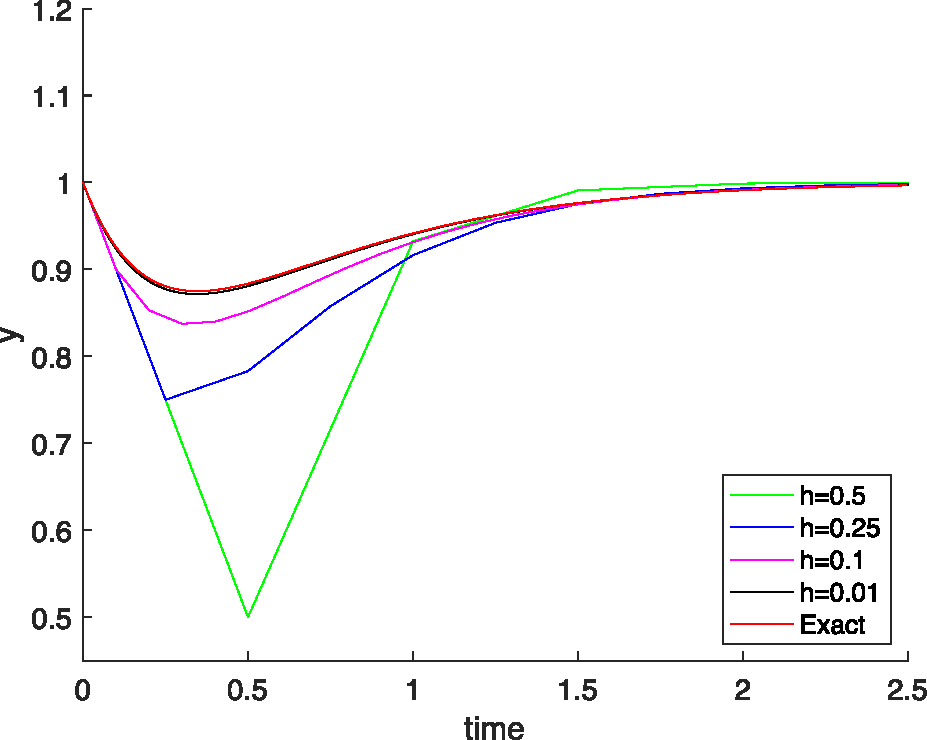
\includegraphics[scale=0.5]{files/exampleEuler.pdf}
    \caption{Results for smaller step sizes using Euler's method.}
    \label{fig:eulerHs}
\end{figure}

Notice that the approximation fits the exact curve as the step size is reduced. In order to illustrate the that Euler's method fails for certain type of differential equations, we shall present the following examples.

\begin{exmp}
Solve the following initial value problem using Euler's method \cite{exampleeuler}.
\begin{equation}
\begin{cases}
    y'-y=-\dfrac{1}{2}e^{\frac{t}{2}}\sin(5t)+5e^{\frac{t}{2}}\cos(5t)&\\ y(0)=0\quad t\in[0,7.5]&
\end{cases}
\end{equation}\label{eq:ex2euler}
\end{exmp}
Applying analytic procedures, the exact solution is given by
\begin{equation}
    y=e^{\frac{t}{2}}\sin(5t)
\end{equation}
In order to apply Euler's method, equation \eqref{eq:ex2euler} can be written as 
\begin{equation}
    y'= y-\dfrac{1}{2}e^{\frac{t}{2}}\sin(5t)+5e^{\frac{t}{2}}\cos(5t)
\end{equation}
As we have the same form as equation \eqref{eq:iode}, we may apply Euler's method with $f(t,y)=y-\dfrac{1}{2}e^{\frac{t}{2}}\sin(5t)+5e^{\frac{t}{2}}\cos(5t)$ and different step sizes to show the results. 

In table \ref{tab:ex2euler}, the results for different time steps and sampling for $t=1,...,7$, and in figure \ref{fig:ex2euler}.

\begin{table}[H]
\centering
\begin{tabular}{cccccc}
\hline
\textbf{Time}         & \textbf{\boldmath$h=0.5$} & \textbf{\boldmath$h=0.25$} & \textbf{\boldmath$h=0.1$} & \textbf{\boldmath$h=0.01$} & \textbf{Exact} \\ \hline
\boldmath{$t=0$} & 0&0&0&0&0\\
\boldmath{$t=1$} & 2.5000                    & 0.9615                     & -0.8028                   & -1.5278                    & -1.5810        \\
\boldmath{$t=2$} & 3.0437                    & 4.4541                     & 1.7565                    & -1.1177                    & -1.4788        \\
\boldmath{$t=3$} & 3.5231                    & 7.8287                     & 7.5072                    & 3.5863                     & 2.9144         \\
\boldmath{$t=4$} & 11.8335                   & 10.5377                    & 11.7976                   & 7.6874                     & 6.7458         \\
\boldmath{$t=5$} & 39.3181                   & 25.9843                    & 15.3996                   & 0.9441                     & -1.6124        \\
\boldmath{$t=6$} & 89.7192                   & 86.9894                    & 46.5853                   & -10.5407                   & -19.8451       \\
\boldmath{$t=7$} & 168.5382                  & 233.7051                   & 168.3623                  & 13.1961                    & -14.1795       \\ \hline
\end{tabular}
\caption{Numerical results using Euler's method and different step sizes.}
\label{tab:ex2euler}
\end{table}

\begin{figure}[H]
    \centering
    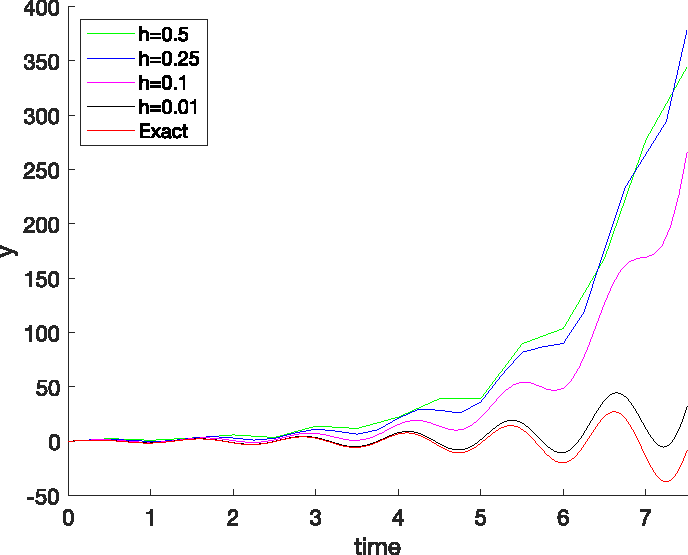
\includegraphics[scale=0.5]{files/example2Euler.pdf}
    \caption{Plots for the Euler's numerical approach with different time steps.}
    \label{fig:ex2euler}
\end{figure}

\begin{exmp}
Solve the following initial value problem using Euler's method.
\begin{equation}
\begin{cases}
    y' = 10e^{-\frac{(t-2)^2}{2}}\left(10\cos(10t)-(t-2)\sin(10t)\right)&\\ y(0) = 0 \quad t\in[0,7.5]&
\end{cases}
\end{equation}
\end{exmp}

The exact solution to this differential equation can be easily obtained and is given by

\begin{equation}
    y(t) = 10e^{-\frac{(t-2)^2}{2}}\sin(10t)
\end{equation}

As the previous examples, table \ref{tab:ex3euler} and figure \ref{fig:ex3euler} show the numeric solution using different time steps.

\begin{table}[H]
\centering
\begin{tabular}{cccccc}
\hline
\textbf{Time}           & \textbf{\boldmath$h=0.5$} & \textbf{\boldmath$t=0.25$} & \textbf{\boldmath$t=0.1$} & \textbf{\boldmath$t=0.01$} & \textbf{Exact} \\ \hline
\textbf{\boldmath$t=0$} & 0                    & 0                     & 0                    & 0                    & 0        \\
\textbf{\boldmath$t=1$} & 6.7668                    & 0.7530                     & 4.9597                    & -2.3979                    & -3.2997        \\
\textbf{\boldmath$t=2$} & -18.0595                  & -4.7931                    & -2.9158                   & 8.4869                     & 9.1295         \\
\textbf{\boldmath$t=3$} & -29.7418                  & 11.2838                    & -1.0473                   & -6.0916                    & -5.9927        \\
\textbf{\boldmath$t=4$} & 21.9611                   & -2.0837                    & 2.0016                    & 1.2339                     & 1.0084         \\
\textbf{\boldmath$t=5$} & 2.8130                    & 1.6074                     & 0.4535                    & 0.0203                     & -0.0291        \\
\textbf{\boldmath$t=6$} & 4.0794                    & 1.3343                     & 0.6358                    & 0.0666                     & -0.0010        \\
\textbf{\boldmath$t=7$} & 4.1062                    & 1.3357                     & 0.6300                    & 0.0672                     & 0.0000         \\ \hline
\end{tabular}
\caption{Numerical results using Euler's method for different step sizes.}
\label{tab:ex3euler}
\end{table}

\begin{figure}[H]
    \centering
    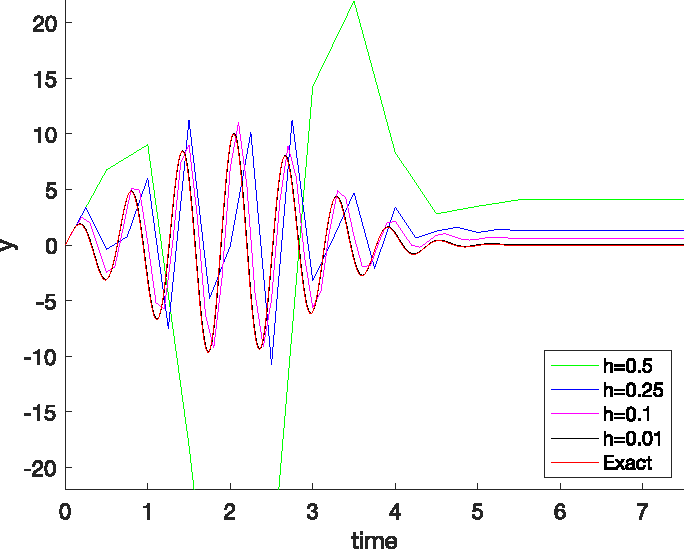
\includegraphics[scale=0.5]{files/example3Euler.pdf}
    \caption{Plots for numerical approach.}
    \label{fig:ex3euler}
\end{figure}

Notice that this differential equation describes an stable system, yet it does not fit the exact solution in stationary state; even with $h=0.1$, the numeric approximation does not stabilizes in the same value.

The previous two examples shows that Euler's method fails for functions that change rapidly and the approximation starts to separate from the exact solution. In order to obtain more exact approximations, we shall present the following numeric method.
